%% IMPORTANT: The official thesis specifications are available at:
%%            http://libraries.mit.edu/archives/thesis-specs/
%%
%%            Please verify your thesis' formatting and copyright
%%            assignment before submission.  If you notice any
%%            discrepancies between these templates and the
%%            MIT Libraries' specs, please let us know
%%            by e-mailing thesis@mit.edu

%% The documentclass options along with the pagestyle can be used to generate
%% a technical report, a draft copy, or a regular thesis.  You may need to
%% re-specify the pagestyle after you \include  cover.tex.  For more
%% information, see the first few lines of mitthesis.cls.

%\documentclass[12pt,vi,twoside]{mitthesis}
%%
%%  If you want your thesis copyright to you instead of MIT, use the
%%  ``vi'' option, as above.
%%
%\documentclass[12pt,twoside,leftblank]{mitthesis}
%%
%% If you want blank pages before new chapters to be labelled ``This
%% Page Intentionally Left Blank'', use the ``leftblank'' option, as
%% above.

\documentclass[12pt,twoside]{mitthesis}
\usepackage{lgrind}
\pagestyle{plain}

%% This bit allows you to either specify only the files which you wish to
%% process, or `all' to process all files which you \include.
%% Krishna Sethuraman (1990).

% \typein [\files]{Enter file names to process, (chap1,chap2 ...), or `all' to
% process all files:}
% \def\all{all}
% \ifx\files\all \typeout{Including all files.} \else \typeout{Including only \files.} \includeonly{\files} \fi

\def\thetitle{Realization of Bose-Einstein Condensation with Lithium-$7$ Atoms}

\usepackage[pdftex,pdfauthor={Yichao Yu},pdftitle={\thetitle}]{hyperref}

\usepackage{amsmath}
\usepackage{amssymb}
\usepackage{amsfonts}

\newcommand{\ud}{\mathrm{d}}
\newcommand{\ue}{\mathrm{e}}
\newcommand{\ui}{\mathrm{i}}
\newcommand{\res}{\mathrm{Res}}
\newcommand{\Tr}{\mathrm{Tr}}
\newcommand{\dsum}{\displaystyle\sum}
\newcommand{\dprod}{\displaystyle\prod}
\newcommand{\dlim}{\displaystyle\lim}
\newcommand{\dint}{\displaystyle\int}
\newcommand{\fsno}[1]{{\!\not\!{#1}}}
\newcommand{\eqar}[1]
{
  \begin{align*}
    #1
  \end{align*}
}
\newcommand{\texp}[2]{\ensuremath{{#1}\times10^{#2}}}
\newcommand{\dexp}[2]{\ensuremath{{#1}\cdot10^{#2}}}
\newcommand{\eval}[2]{{\left.{#1}\right|_{#2}}}
\newcommand{\paren}[1]{{\left({#1}\right)}}
\newcommand{\lparen}[1]{{\left({#1}\right.}}
\newcommand{\rparen}[1]{{\left.{#1}\right)}}
\newcommand{\abs}[1]{{\left|{#1}\right|}}
\newcommand{\sqr}[1]{{\left[{#1}\right]}}
\newcommand{\crly}[1]{{\left\{{#1}\right\}}}
\newcommand{\angl}[1]{{\left\langle{#1}\right\rangle}}
\newcommand{\tpdiff}[4][{}]{{\paren{\frac{\partial^{#1} {#2}}{\partial {#3}{}^{#1}}}_{#4}}}
\newcommand{\tpsdiff}[4][{}]{{\paren{\frac{\partial^{#1}}{\partial {#3}{}^{#1}}{#2}}_{#4}}}
\newcommand{\pdiff}[3][{}]{{\frac{\partial^{#1} {#2}}{\partial {#3}{}^{#1}}}}
\newcommand{\diff}[3][{}]{{\frac{\ud^{#1} {#2}}{\ud {#3}{}^{#1}}}}
\newcommand{\psdiff}[3][{}]{{\frac{\partial^{#1}}{\partial {#3}{}^{#1}} {#2}}}
\newcommand{\sdiff}[3][{}]{{\frac{\ud^{#1}}{\ud {#3}{}^{#1}} {#2}}}
\newcommand{\tpddiff}[4][{}]{{\left(\dfrac{\partial^{#1} {#2}}{\partial {#3}{}^{#1}}\right)_{#4}}}
\newcommand{\tpsddiff}[4][{}]{{\paren{\dfrac{\partial^{#1}}{\partial {#3}{}^{#1}}{#2}}_{#4}}}
\newcommand{\pddiff}[3][{}]{{\dfrac{\partial^{#1} {#2}}{\partial {#3}{}^{#1}}}}
\newcommand{\ddiff}[3][{}]{{\dfrac{\ud^{#1} {#2}}{\ud {#3}{}^{#1}}}}
\newcommand{\psddiff}[3][{}]{{\frac{\partial^{#1}}{\partial{}^{#1} {#3}} {#2}}}
\newcommand{\sddiff}[3][{}]{{\frac{\ud^{#1}}{\ud {#3}{}^{#1}} {#2}}}

\usepackage{tikz}
\usetikzlibrary{
  arrows,
  calc,
  decorations.pathmorphing,
  decorations.pathreplacing,
  decorations.markings,
  fadings,
  positioning,
  shapes,
  3d
}
\tikzset{snake arrow/.style={->,
    decorate,
    decoration={snake,amplitude=.4mm,segment length=2mm,post length=1mm}},
}
\tikzset{
  partial ellipse/.style args={#1:#2:#3}{
    insert path={+ (#1:#3) arc (#1:#2:#3)}
  }
}

\usepackage{subfigure}


\begin{document}

% -*-latex-*-
%
% For questions, comments, concerns or complaints:
% thesis@mit.edu
%
%
% $Log: cover.tex,v $
% Revision 1.8  2008/05/13 15:02:15  jdreed
% Degree month is June, not May.  Added note about prevdegrees.
% Arthur Smith's title updated
%
% Revision 1.7  2001/02/08 18:53:16  boojum
% changed some \newpages to \cleardoublepages
%
% Revision 1.6  1999/10/21 14:49:31  boojum
% changed comment referring to documentstyle
%
% Revision 1.5  1999/10/21 14:39:04  boojum
% *** empty log message ***
%
% Revision 1.4  1997/04/18  17:54:10  othomas
% added page numbers on abstract and cover, and made 1 abstract
% page the default rather than 2.  (anne hunter tells me this
% is the new institute standard.)
%
% Revision 1.4  1997/04/18  17:54:10  othomas
% added page numbers on abstract and cover, and made 1 abstract
% page the default rather than 2.  (anne hunter tells me this
% is the new institute standard.)
%
% Revision 1.3  93/05/17  17:06:29  starflt
% Added acknowledgements section (suggested by tompalka)
%
% Revision 1.2  92/04/22  13:13:13  epeisach
% Fixes for 1991 course 6 requirements
% Phrase "and to grant others the right to do so" has been added to
% permission clause
% Second copy of abstract is not counted as separate pages so numbering works
% out
%
% Revision 1.1  92/04/22  13:08:20  epeisach

% NOTE:
% These templates make an effort to conform to the MIT Thesis specifications,
% however the specifications can change.  We recommend that you verify the
% layout of your title page with your thesis advisor and/or the MIT
% Libraries before printing your final copy.
\title{\thetitle}

\author{Yichao Yu}
% If you wish to list your previous degrees on the cover page, use the
% previous degrees command:
%       \prevdegrees{A.A., Harvard University (1985)}
% You can use the \\ command to list multiple previous degrees
%       \prevdegrees{B.S., University of California (1978) \\
%                    S.M., Massachusetts Institute of Technology (1981)}
\department{Department of Physics}

% If the thesis is for two degrees simultaneously, list them both
% separated by \and like this:
% \degree{Doctor of Philosophy \and Master of Science}
\degree{Bachelor of Science in Physics}

% As of the 2007-08 academic year, valid degree months are September,
% February, or June.  The default is June.
\degreemonth{June}
\degreeyear{2014}
\thesisdate{May 18, 2014}

%% By default, the thesis will be copyrighted to MIT.  If you need to copyright
%% the thesis to yourself, just specify the `vi' documentclass option.  If for
%% some reason you want to exactly specify the copyright notice text, you can
%% use the \copyrightnoticetext command.
%\copyrightnoticetext{\copyright IBM, 1990.  Do not open till Xmas.}

% If there is more than one supervisor, use the \supervisor command
% once for each.
\supervisor{Wolfgang Ketterle}{Professor}

% This is the department committee chairman, not the thesis committee
% chairman.  You should replace this with your Department's Committee
% Chairman.
\chairman{Nergis Mavalvala}{Senior Thesis Coordinator, Department of Physics}

% Make the titlepage based on the above information.  If you need
% something special and can't use the standard form, you can specify
% the exact text of the titlepage yourself.  Put it in a titlepage
% environment and leave blank lines where you want vertical space.
% The spaces will be adjusted to fill the entire page.  The dotted
% lines for the signatures are made with the \signature command.
\maketitle

% The abstractpage environment sets up everything on the page except
% the text itself.  The title and other header material are put at the
% top of the page, and the supervisors are listed at the bottom.  A
% new page is begun both before and after.  Of course, an abstract may
% be more than one page itself.  If you need more control over the
% format of the page, you can use the abstract environment, which puts
% the word "Abstract" at the beginning and single spaces its text.

%% You can either \input (*not* \include) your abstract file, or you can put
%% the text of the abstract directly between the \begin{abstractpage} and
%% \end{abstractpage} commands.

% First copy: start a new page, and save the page number.
\cleardoublepage
% Uncomment the next line if you do NOT want a page number on your
% abstract and acknowledgments pages.
% \pagestyle{empty}
\setcounter{savepage}{\thepage}
\begin{abstractpage}
% $Log: abstract.tex,v $
% Revision 1.1  93/05/14  14:56:25  starflt
% Initial revision
%
% Revision 1.1  90/05/04  10:41:01  lwvanels
% Initial revision
%
%
%% The text of your abstract and nothing else (other than comments) goes here.
%% It will be single-spaced and the rest of the text that is supposed to go on
%% the abstract page will be generated by the abstractpage environment.  This
%% file should be \input (not \include 'd) from cover.tex.
Ultra-cold atoms are atoms that are at a temperature close to absolute zero, typically at the order of micro Kelvin or lower. At these low temperatures, the quantum properties of the atoms, which are usually dominated by thermal effect at room temperature ($\approx300K$), becomes important and the atoms can form interesting new states of matter including Bose-Einstein condensation (BEC) for bosons and degenerate Fermi gas for fermions.\\
\\
This thesis presents our work on developing and improving the techniques of trapping and cooling an ultra-cold cloud of Lithium-$7$ atoms and the realization of the Bose-Einstein condensation. The techniques used in this experiment includes Zeeman slower, magneto-optical trap (MOT), gray molasses, static magnetic trap, evaporative cooling, optical dipole trap (ODT), etc.

\end{abstractpage}

% Additional copy: start a new page, and reset the page number.  This way,
% the second copy of the abstract is not counted as separate pages.
% Uncomment the next 6 lines if you need two copies of the abstract
% page.
% \setcounter{page}{\thesavepage}
% \begin{abstractpage}
% % $Log: abstract.tex,v $
% Revision 1.1  93/05/14  14:56:25  starflt
% Initial revision
%
% Revision 1.1  90/05/04  10:41:01  lwvanels
% Initial revision
%
%
%% The text of your abstract and nothing else (other than comments) goes here.
%% It will be single-spaced and the rest of the text that is supposed to go on
%% the abstract page will be generated by the abstractpage environment.  This
%% file should be \input (not \include 'd) from cover.tex.
Ultra-cold atoms are atoms that are at a temperature close to absolute zero, typically at the order of micro Kelvin or lower. At these low temperatures, the quantum properties of the atoms, which are usually dominated by thermal effect at room temperature ($\approx300K$), becomes important and the atoms can form interesting new states of matter including Bose-Einstein condensation (BEC) for bosons and degenerate Fermi gas for fermions.\\
\\
This thesis presents our work on developing and improving the techniques of trapping and cooling an ultra-cold cloud of Lithium-$7$ atoms and the realization of the Bose-Einstein condensation. The techniques used in this experiment includes Zeeman slower, magneto-optical trap (MOT), gray molasses, static magnetic trap, evaporative cooling, optical dipole trap (ODT), etc.

% \end{abstractpage}

\cleardoublepage

\section*{Acknowledgments}

% TODO
% This is the acknowledgements section.  You should replace this with your
% own acknowledgements.

%%%%%%%%%%%%%%%%%%%%%%%%%%%%%%%%%%%%%%%%%%%%%%%%%%%%%%%%%%%%%%%%%%%%%%
% -*-latex-*-

% Some departments (e.g. 5) require an additional signature page.  See
% signature.tex for more information and uncomment the following line if
% applicable.
% % -*- Mode:TeX -*-
%
% Some departments (e.g. Chemistry) require an additional cover page
% with signatures of the thesis committee.  Please check with your
% thesis advisor or other appropriate person to determine if such a 
% page is required for your thesis.  
%
% If you choose not to use the "titlepage" environment, a \newpage
% commands, and several \vspace{\fill} commands may be necessary to
% achieve the required spacing.  The \signature command is defined in
% the "mitthesis" class
%
% The following sample appears courtesy of Ben Kaduk <kaduk@mit.edu> and
% was used in his June 2012 doctoral thesis in Chemistry. 

\begin{titlepage}
\begin{large}
This doctoral thesis has been examined by a Committee of the Department
of Chemistry as follows:

\signature{Professor Jianshu Cao}{Chairman, Thesis Committee \\
   Professor of Chemistry}

\signature{Professor Troy Van Voorhis}{Thesis Supervisor \\
   Associate Professor of Chemistry}

\signature{Professor Robert W. Field}{Member, Thesis Committee \\
   Haslam and Dewey Professor of Chemistry}
\end{large}
\end{titlepage}


\pagestyle{plain}
  % -*- Mode:TeX -*-
%% This file simply contains the commands that actually generate the table of
%% contents and lists of figures and tables.  You can omit any or all of
%% these files by simply taking out the appropriate command.  For more
%% information on these files, see appendix C.3.3 of the LaTeX manual.
\tableofcontents
\newpage
\listoffigures
\newpage
\listoftables

\chapter{Introduction}

Predicted in 1924-25 by Satyendra Nath Bose and Albert Einstein from Bose statistics, the Bose Einstein condensate is a phase of matter at ultra-cold temperature that emerges completely because of quantum effects. It was first produced in the laboratory in 1995-96 at the University of Colorado Boulder, Massachusetts Institute of Technology and Rice University using laser cooling and evaporative cooling techniques. Since then, people have been using it to study many quantum effects. Among them, one effort is to simulate complex condensed matter systems using simplfied and well controlled model systems created by loading BEC into optical lattices.\\
\\
In our experiment, we use the Lithium-$7$ atoms to create a Bose-Einstein condensate. Because of the lightness and several Feshbach resonances, the Lithium-$7$ atom has very fast dynamics and great tunability, making it a perfect candidate for simulating and studying the phase diagrams of certain condensed matter models. The ultimate goal of the experiment is to study the anti-ferromagnetic phase in the anisotropic Heisenberg model ($XXZ$ model), and the work in this thesis focuses on getting a Bose-Einstein condensate using Lithium-$7$, which is one of the important steps before studying the system in an optical lattice.\\
\\
The presentation of this thesis is divided into two chapters. In the first chapter, I discuss the theory of our experiment, including the Bose-Einstein condensate (BEC) and the various cooling and trapping techniques we use. The second chapter describes the setup of the experiment, the alignment and optimization procedure we developed and the experimental results we have got for each steps.

\chapter{Theory}

In this chapter, I am going to describe the theories behind our experiment. It is divided into three parts. The first section explains the theories of cold Bose gas and the Bose-Einstein condensation relevant to the experiment. The second section briefly describes some important properties of the Lithium-$7$ atom. Finally, in the third section, the cooling, trapping and state manipulation techniques used in the experiment are presented, including Zeeman slower (\ref{theory:zeeman}), MOT(\ref{theory:mot}), gray molasses (\ref{theory:gm}), dark state pumping (\ref{theory:pump}), magnetic trap (\ref{theory:mt}) and optical dipole trap (\ref{theory:odt}).

\section{What is Bose-Einstein Condensate}\label{theory:bec}

Every real particles can be classified as one of the two families according to their spins, fermions which have half integer spins and bosons which have integer spins. According to quantum field theory\cite{spin-statistics1,spin-statistics2} the many-particles wave function of identical particles must be symmetric or anti-symmetric under particle exchange for bosons or fermions respectively. For bosonic particles, because of the symmetry of the wave function, the possibility for particles to be in the same state is greatly enhances. As a result, boson gas at ultra-low temperature forms a Bose-Einstein condensate (BEC), in which almost all of the particles are condensed to the lowest energy state. In the following, the relevant properties of BECs such as critical temperature and density distribution are described.

\subsection{BEC in Harmonic Trap}

Since the wave function of bosons is symmetric, multiple bosons can be in the same state. From this fact, the energy distribution can be calculated for bosons,
\eqar{
  f(\varepsilon)=&\frac{1}{\ue^{\beta(\varepsilon-\mu)} - 1}
}
Since the distribution has to be possitive for all energy states, in particular the $\varepsilon=0$ ground state, we have $\mu\geqslant0$. For all the state except the ground state, this sets an finite upper limit on the number of atoms in each state for a fixed temperature. Therefore, if the number of atoms exceeds a certain value, all the extra atoms will go into the ground state. These atoms condensed in the ground state are called the Bose Einstein condensate.\\
\\
In order to calculate the atom number in the condensate as well as the critical temperature, we can estimate the maximum atom number in the excited states (thermal atoms) with an integral,
\eqar{
  N_{th}=&\int_0^\infty\frac{g(\varepsilon)}{\ue^{\beta\varepsilon} - 1}\ud\varepsilon
}
where $g(\varepsilon)$ is the energy density of states. In our experiment, we create the BEC in a harmonic optical dipole trap (see \ref{theory:odt}) for which the energy density is,
\eqar{
  g(\varepsilon)=&\frac{\varepsilon^2}{2\hbar^3 \omega^3}\\
  N_{th}=&\frac{1}{2\hbar^3 \omega^3}\int_0^\infty\frac{\varepsilon^2}{\ue^{\beta\varepsilon} - 1}\ud\varepsilon\\
  =&\frac{1}{2\hbar^3 \omega^3\beta^3}\int_0^\infty\frac{x^2}{\ue^{x} - 1}\ud x\\
  =&\frac{k_B^3T^3}{2\hbar^3 \omega^3}\zeta(3)\Gamma(3)
}
The critical temperature of the transition, determined by $N_{th}=N$,
\eqar{
  T_C=&\frac{\hbar\omega}{k_B}\sqrt[3]{\frac{2N}{\zeta(3)\Gamma(3)}}\\
  =&0.9405\frac{\hbar\omega\sqrt[3]{N}}{k_B}
}
Condensate fraction (for large $N$),
\eqar{
  \frac{N_0}{N}=&1-\frac{N_{th}}{N}\\
  =&1-\paren{\frac{T}{T}}^3
}

\subsection{Effect of interaction}

The wavefunction of the condensed atoms is only the same with the single particle ground state wavefunction when there is no interaction between atoms. For interacting Bose gas this is no longer true. The

The ... only works for non-interacting.... when adding in interaction.... change shape..... this sub section describe .... in order to measure ....

\section{Lithium-$7$ Atoms}

Fine structure\\
Hyperfine structure\\
Zeeman effect

\begin{table}
\caption{$g$-factors of Lithium-$7$}
\label{li7:g-factors}
\begin{center}
\begin{tabular}{|c|c|c|}\hline
Fine Structure & $F$ & $g$-factor \\\hline
$2^2S_{1/2}$ & $2$ & $\dfrac 12$ \\\cline{2-3}
 & $1$ & $-\dfrac 12$ \\\hline
$2^2P_{1/2}$ & $2$ & $\dfrac 16$ \\\cline{2-3}
 & $1$ & $-\dfrac 16$ \\\hline
$2^2P_{3/2}$ & $1$, $2$, $3$ & $\dfrac 23$ \\\hline
\end{tabular}
\end{center}
\end{table}

% TODO high field Zeeman

\section{Cooling and Traping Theory}

The atoms used in an alkali atom experiment often come from an atom beam coming out of a oven kept above the melting temperature of the metal. The oven used in this experiment operates at $485^\circ\text{C}$ producing an atom beam traveling at several hundred meters per second. In order to achieve low temperature and high density, several stages of slowing, traping and cooling are implemented in this experiment which finally bring the atoms down to the Bose-Einstein condensate condition. In this section, I am going to talk about the theory behind these techniques we are using in our experiment.

\subsection{Zeeman Slower}\label{theory:zeeman}

The atoms comes out of the oven has an average velocity determined by the Maxwell-Boltzmann distribution,
\eqar{
  \bar v=&\sqrt{\frac{k_BT}{2\pi m}}
}
We can slow down the atoms using the recoil of photon scattering by shining resonance light to the beam. However, since the atomic transition resonance is very narrow ($\Gamma=2\pi\cdot5.9\text{MHz}$) compare to the doppler shift ($\Delta\nu=\nu v/c\approx590\text{MHz}$), the atom will soon shift out of resonance once it slows down. There are several ways to solve this problem. One way is to modulate the laser frequency, either swiping with time (frequency chriping) or making it broadband (white light). The Zeeman slower solves the problem by changing the resonance of the atom with Zeeman effect. This is the most popular way for alkali atoms which usually have a cycling transition with linear Zeeman effect in a large range.\\
\\
The Zeeman slower has a magnetic field aligned with the atom beam with a spacially variant amplitude. By shining circularly polarized light against the atom beam, the atoms in the beam are optically pumped to one of the two stretch states determined by the relative direction of the field and the light polarization. If the magnetic field is changing in a way such that the Zeeman shift of the atom follows the Doppler shift when atoms slow down, the atom beam will be always in resonance and continuously being slowed down, i.e.
\eqar{
  g_Fm_F\mu_BB=\frac{v}{c}\nu+\Delta
}
For constant acceleration, this implies,
\eqar{
  B=\frac{\sqrt{v_0^2-2ax}}{g_Fm_F\mu_Bc}\nu+B_0
}
The maximum deceleration of the Zeeman slower is limited by the maximum scattering rate, therefore the life time of the excited state,
\eqar{
  a_{max}=&\frac{h\Gamma}{2\lambda}
}
where $\Gamma$ is the linewidth of the transition.

\subsection{Magneto-Optical Trap (MOT)}\label{theory:mot}

As in most cold atom experiment, our experiment starts with loading Zeeman slowed atom into a magneto-optical trap (MOT). MOT is a technique that uses laser and magnetic field gradient to provides both molasses cooling and confinement. In order to understand how MOT works, we can consider a one-dimensional model.\\
\\
The one-dimensinal model consists of a spacially varying magnetic field $B=B'x$, two counter propagating, red-detuned, circularly polarized light with atoms sitting close to the zero of the magnetic field.

\subsection{Gray Molasses}\label{theory:gm}

\subsection{Dark State Pumping}\label{theory:pump}
At the end of Laser cooling, the atoms are distributed in different ground states.\\
In order to trap in MT, need to go to 2, 2 / 2, 1 which are the only trappable states at both low field and high field.\\
Choose 2, 2 because we can use dark state pumping which ...

Dark State pumping with D1 light

\subsection{Evaporation in Static Magnetic Trap}\label{theory:mt}
Trapable states
Power law?

\subsection{Evaporation in Optical Dipole Trap}\label{theory:odt}
AC Stark Shift
Cross ODT
Feshbach resonance

\chapter{Experimental Setup and Results}

In this chapter, I will describe our experimental setup and results. It includes a brief discussion of our optical tables setup (\ref{exp:laser-table} and \ref{exp:machine-table}), the implementation, optimization and performance of each steps (\ref{exp:mot}, \ref{exp:gm}, \ref{exp:pump}, \ref{exp:mt} and \ref{exp:odt}) and finally some basic characteristic of our BEC (\ref{exp:odt}).

\section{Laser System}\label{exp:laser-table}
The laser table is where we prepare all the light resonance with the Lithium-$7$ transition ($\approx671nm$). As discussed in the previous chapter, there are four distinct lines that we need in the experiment, the combination of $D1$, $D2$ with $F1$, $F2$. At a certain time, we need either $D1$ or $D2$ light with the probability of using both $F1$ and $F2$ at the same time and the laser table is designed to do just this.\\
\begin{figure}
  \begin{center}
    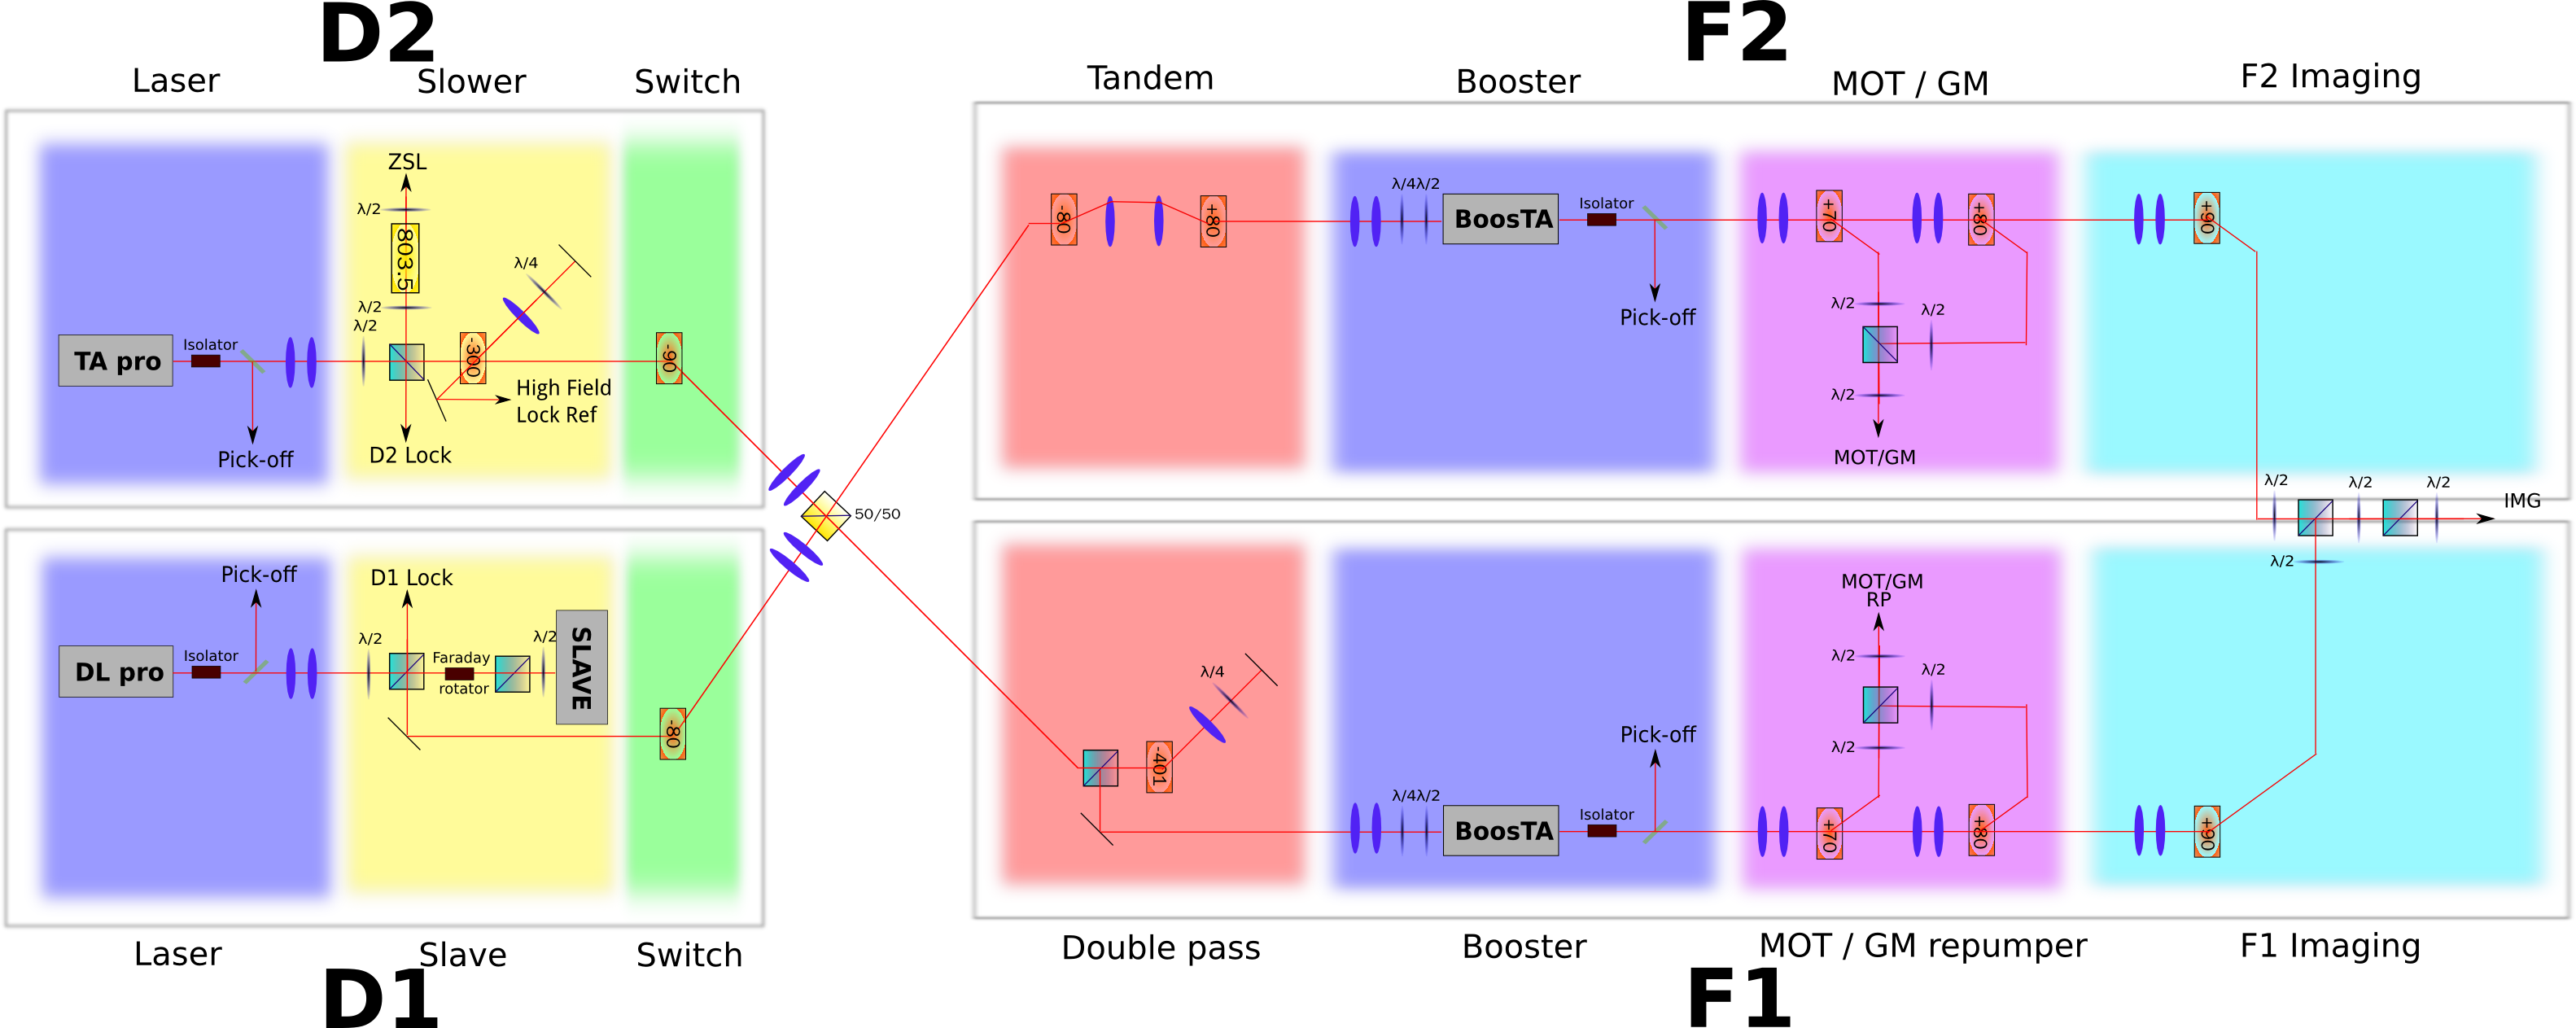
\includegraphics[width=14cm]{laser_table.png}
  \end{center}
  \caption{Schematic of the laser table design}
  \label{exp:laser-table-design}
\end{figure}\\
As shown in figure \ref{exp:laser-table-design}, since the separation between the $D1$ and $D2$ line ($\approx10GHz$) is larger than the range of common optical frequency shifters (e.g. AOMs), the $D1$ and $D2$ light are created separately using two diode lasers (TA pro and DL pro in figure \ref{exp:laser-table-design}). Both of these lasers are actively locked to the appropriate atomic transitions using saturated absorption spectroscopy to better than $2\text{MHz}$. For the $D2$ path, part of the light ($\approx80mW$) is red shifted and used as the Zeeman slower light ($ZSL$ in the figure) and the rest goes to the $D2$, $D1$ selecting switch, which uses two AOMs (acousto-optical modulator) and a $50$-$50$ cube to feed both the $F1$ and $F2$ path with either $D1$ and $D2$ light. For the $D1$ path, a slave diode is used to amplify the light before going to the switch.\\
\\
In the $F1$, $F2$ path, a tandem and a double pass are used to continuously shift the frequency of the laser (the double pass is also used to shift the light from $F2$ to $F1$). After that, the light in each path is amplified using tapered amplifier and then go through a polarization switch consists of two AOMs and a polarization beam splitter which can but the light into polarization maintaining fibers (MOT/GM and MOT/GM RP) with two orthogonal linear polarization's (the use of these beams is further described in section \ref{exp:mot-cage}). At the end of the chain, two more AOMs are used to control the light we put into the imaging fiber so that we can image on any of the four transitions. Each fibers also has a mechanical shutter that is used to block any possible leaking light that may cause heating.

\section{Vacuum Chamber and Main Coils Configuration}\label{exp:machine-table}

In this section, I am going to describe some important setup on the machine table where out vacuum chamber sits on.

\subsection{Optical Access of the Vacuum Chamber}\label{exp:chamber}
The windows and connections except the top and bottom window on our main vacuum chamber is shown in figure \ref{chamber-light}. There are in total $6$ MOT/Gray Molasses beams, $2$ ODT beams, $3$ Imaging beams, a plug and a Zeeman slower beam going into the chamber. When multiple colors need to be sent in through the same window, they are combined outside the vacuum chamber using appropriate dichroic.
\begin{figure}
  \begin{center}
    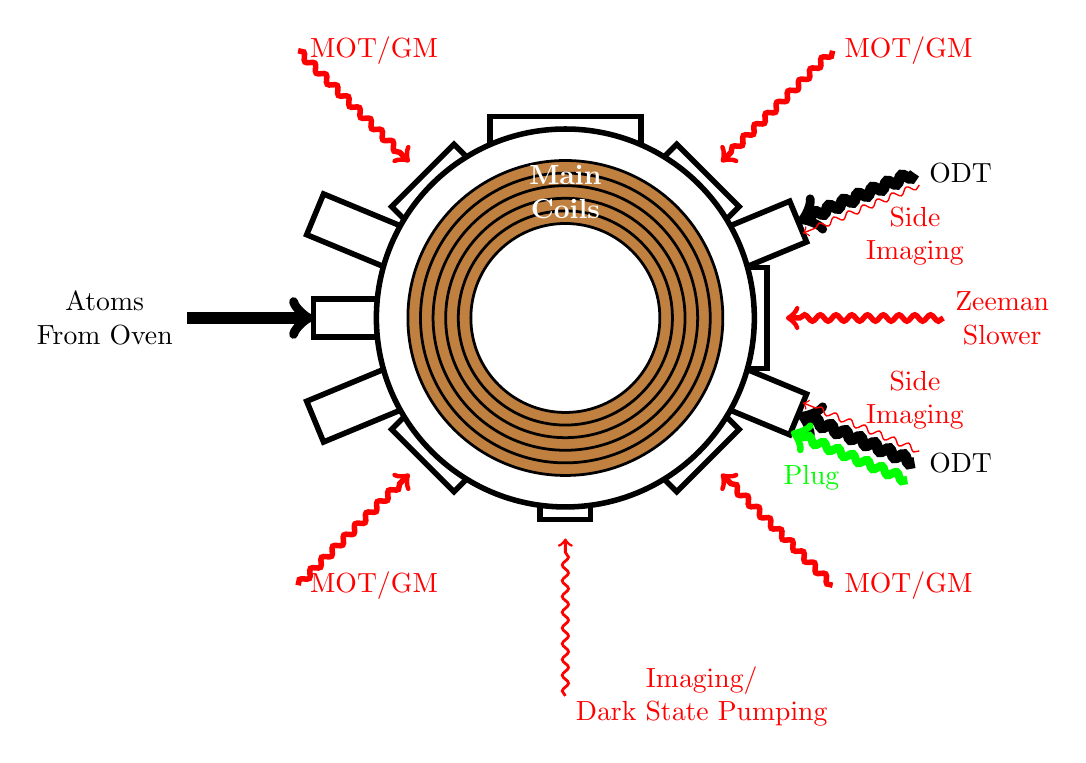
\begin{tikzpicture}[scale=0.8]
      % ODT windows
      \draw[rotate around={22.5:(0, 0)},line width=2] (-4.3, -.35) rectangle (4, .35);
      \draw[rotate around={-22.5:(0, 0)},line width=2] (-4.3, -.35) rectangle (4, .35);

      % MOT windows
      \draw[rotate around={45:(0, 0)},line width=2] (-3.2, -.7) rectangle (3.2, .7);
      \draw[rotate around={-45:(0, 0)},line width=2] (-3.2, -.7) rectangle (3.2, .7);

      % Slower windows
      \draw[line width=2] (0, -.8) rectangle (3.2, .8);
      \draw[line width=2] (-4, -.3) rectangle (0, .3);

      % Imaging windows
      \draw[line width=2] (-1.2, 0) rectangle (1.2, 3.2);
      \draw[line width=2] (-.4, 0) rectangle (.4, -3.2);

      % Main Chamber
      \draw[fill=white,line width=2] (0, 0) circle (3);

      % Coils
      \draw[line width=1,fill=brown] (0, 0) circle (2.5);
      \draw[line width=1] (0, 0) circle (2.3);
      \draw[line width=1] (0, 0) circle (2.1);
      \draw[line width=1] (0, 0) circle (1.9);
      \draw[line width=1] (0, 0) circle (1.7);
      \draw[line width=1,fill=white] (0, 0) circle (1.5);
      \path (0, 2) node[align=center,white] {\textbf{Main}\\\textbf{Coils}};

      % MOT beams
      \draw[line width=2,snake arrow,rotate around={45:(0, 0)},red] (6, 0) node[right] {MOT/GM} -- ++(-2.5, 0);
      \draw[line width=2,snake arrow,rotate around={-45:(0, 0)},red] (6, 0) node[right] {MOT/GM} -- ++(-2.5, 0);
      \draw[line width=2,snake arrow,rotate around={135:(0, 0)},red] (6, 0) node[right] {MOT/GM} -- ++(-2.5, 0);
      \draw[line width=2,snake arrow,rotate around={-135:(0, 0)},red] (6, 0) node[right] {MOT/GM} -- ++(-2.5, 0);

      % Imaging
      \draw[line width=1,snake arrow,rotate around={-90:(0, 0)},red] (6, 0) node[right,align=center] {Imaging/\\Dark State Pumping} -- ++(-2.5, 0);

      % ODT1
      \draw[line width=4,snake arrow,rotate around={22.5:(0, 0)}] (6, 0) node[right] {ODT} -- ++(-2, 0);
      \draw[line width=.5,snake arrow,rotate around={22.5:(0, 0)},red] (6, -0.2) -- ++(-2, 0);
      \path[rotate around={22.5:(0, 0)},red] (5, 0) node[below right,align=center] {Side\\Imaging};

      % ODT2
      \draw[line width=4,snake arrow,rotate around={-22.5:(0, 0)}] (6, 0) node[right] {ODT} -- ++(-2, 0);
      \draw[line width=.5,snake arrow,rotate around={-22.5:(0, 0)},red] (6, 0.2) -- ++(-2, 0);
      \path[rotate around={-22.5:(0, 0)},red] (5, 0) node[above right,align=center] {Side\\Imaging};
      \draw[line width=3,snake arrow,rotate around={-22.5:(0, 0)},green] (6, -0.3) -- ++(-2, 0);
      \path[rotate around={-22.5:(0, 0)},green] (5, -0.3) node[below left] {Plug};

      % Slower
      \draw[line width=2,snake arrow,red] (6, 0) node[right,align=center] {Zeeman\\Slower} -- ++(-2.5, 0);
      \draw[line width=4,->,rotate around={180:(0, 0)}] (6, 0) node[left,align=center] {Atoms\\From Oven} -- ++(-2, 0);
    \end{tikzpicture}
  \end{center}
  \caption{Top View of the Vacuum Chamber (Top/Bottom MOT/Gray Molasses beams not included, not to scale).}
  \label{chamber-light}
\end{figure}
\subsection{MOT-Gray Molasses Cage}\label{exp:mot-cage}
The delivery of the MOT and gray molasses beam from the two in-coupler on the laser table to the six output on the machine table is done with a polarization maintaining evanescent wave fiber splitter which takes the light from the two input fibers and split them equally into the six output fibers. However, the MOT beams and the gray molasses beams have different requirement in beam sizes. On one hand, the MOT needs a bigger beam size for a bigger capture volume. On the other hand, as discussed earlier, for the gray molasses to work effectively, high intensity, therefore smaller beam size, is required. In order to have a different size for the two beams coming out of the same fiber, we send in the two beams with orthogonal polarization's (figure \ref{exp:laser-table-design}) and add polarization dependent beam expenders after the fiber output to shape the two beams differently. This beam shaping is done with a cage system shown in figure \ref{mot-cage-design}. The upper beam path is used for expanding the MOT beam whereas the lower path shapes the gray molasses beam to a smaller size. Each of the four lenses can slide in the cage, which are used to tweak the size and divergence of the beams. The alignment between beams is done with the two bottom mirrors and the two half wave-plates between the two polarization beam splitter cubes are used to balance the intensities.
\begin{figure}
  \begin{center}
    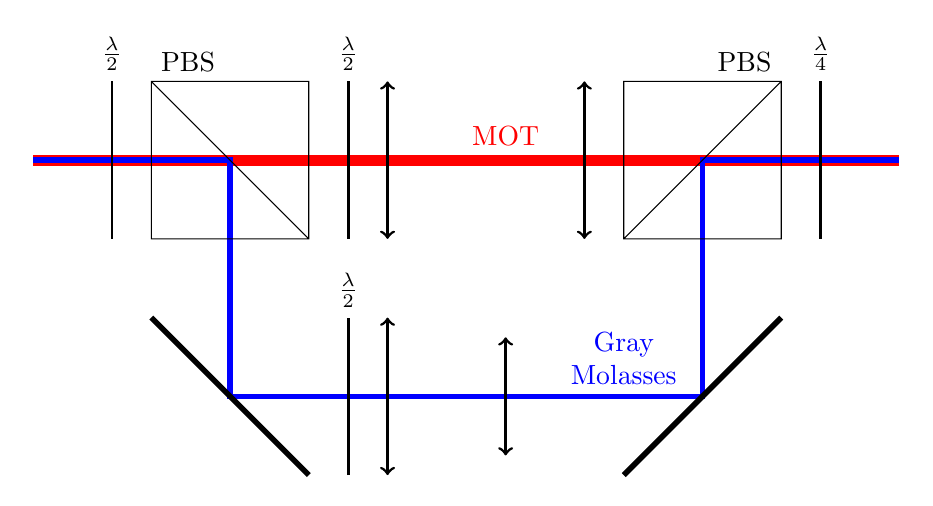
\begin{tikzpicture}
      \draw[line width=4,red] (-1, 1) -- (5, 1) node[above] {MOT} -- (10, 1);

      \draw[line width=2,blue] (-1, 1) -- (1.5, 1) -- ++(0, -3) -- (6.5, -2) node[above,align=center] {Gray\\Molasses} -- (7.5, -2) -- (7.5, 1) -- (10, 1);

      \draw[line width=1] (0, 0) -- ++(0, 2) node[above] {$\frac{\lambda}{2}$};
      \draw (0.5, 2) rectangle ++(2, -2) -- ++(-2, 2) node[above right] {PBS};
      \draw[line width=1] (3, 0) -- ++(0, 2) node[above] {$\frac{\lambda}{2}$};
      \draw[line width=1,<->] (3.5, 0) -- ++(0, 2);
      \draw[line width=1,<->] (6, 0) -- ++(0, 2);
      \draw (6.5, 0) rectangle ++(2, 2) node[above left] {PBS} -- ++(-2, -2);
      \draw[line width=1] (9, 0) -- ++(0, 2) node[above] {$\frac{\lambda}{4}$};

      \draw[line width=2] (2.5, -3) -- ++(-2, 2);
      \draw[line width=1] (3, -3) -- ++(0, 2) node[above] {$\frac{\lambda}{2}$};
      \draw[line width=1,<->] (3.5, -3) -- ++(0, 2);
      \draw[line width=1,<->] (5, -2.75) -- ++(0, 1.5);
      \draw[line width=2] (8.5, -1) -- ++(-2, -2);
    \end{tikzpicture}
  \end{center}
  \caption{MOT/Gray Molasses Cage.}
  \label{mot-cage-design}
\end{figure}

\subsection{Main Coils Configuration}\label{exp:coil}
Besides the weak field (up to several Gauss) provided by the shim coils for earth field compensation and small bias field, we use strong magnetic field in the experiment in many different configurations. In the magneto-optical trap, we need a quadrupole field ($\approx20\text{G}\cdot\text{cm}^{-1}$). For the static magnetic trap, we use a stronger quadrupole field ($\approx500\text{G}\cdot\text{cm}^{-1}$). And finally for the evaporation in the optical dipole trap, we need independent control of a very strong bias field (up to $\approx1000\text{G}$) and a gradient on top of it (up to $\approx30\text{G}\cdot\text{cm}^{-1}$). In order to avoid interference between different steps of the experiment, we also need the capability of turning on and off or changing the configuration of the magnetic field quickly ($\ll1\text{ms}$).\\
\\
These strong magnetic field is generated in the experiment by running up to $500\text{A}$ of current through one pair of water cooled coils attached to the vacuum chamber. The coils are positioned closed to the Helmholtz condition to maximize the homogeneity when generating a bias field. Each of the coil consists of $5$ layers which can be connected and powered independently (one of them is damaged during operation and is not used currently) so that they can be used in different configurations. Due to the limitation of our power supplies (both in output capability and in the number we have), many of the field configuration we need requires running current through more than one layer of the coils. Therefore, in order to achieve different configuration of the field, it is necessary to reuse our power supplies and coil layers in different steps.\\
\\
The options available for fast switching of such high current are mechanical relays or solid state (semiconductor) devices. After comparing the performance and reliability of different options, we decided to use high power IGBT's (insulated-gate bipolar transistor) since they are the most widely used solid state device for high current application and can provide a lot shorter response time with similar cost and failing rate compare to mechanical relays. The switching time for these IGBT's to switch certain current are determined by the response time of the device (micro-seconds or shorter) and the maximum voltage they can take (since $\ud I/\ud t=L/U$). Since the IGBT's we use can take a voltage higher than $500\text{V}$, simple calculation shows that they can switch off the maximum current we have within $100\mu s$, which is already much shorter than the decay time of the eddy current in our vacuum chamber (mili-second).\\
\\
In order to generate bias field and quadrupole field with our main coil, we can put current into one pair of layers on both side in the same and opposite direction respectively. However, for reusing a layer, we need to switch the polarity of current on one side and keep the direction on the other side the same. Since each IGBT acts like a single throw single pole switch (in one direction), we need four IGBT's (two on each side) to change the polarity of one layer by connecting the two ends of the layer to either side of the supply. This configuration is called a H-bridge. In addition to this, since each of the four switches are closed only in one case, we can put layers in series with one of the switches so that they are only powered in one of the configurations in order to use different number of layers in the two configurations. After considering other factors including geometrical constraint and convenience the modified H-bridge designed we use in our experiment can be seen in figure \ref{exp:coil-control}. ``Lambda'' and ``Sorenson'' are the two power supplies. Each pair of switch and diode represent an IGBT module with floating TTL input control. The layers are numbered as $1T-4T$ and $1B-4B$ meaning the inner layer to side layers on the top and bottom. The ``in'' and ``out'' labels on the layer terminal represent the direction of the current to generate a quadrupole field. Finally, the blue lines separate the parts on the machine table (coils) and the parts on the power supply rack (power supplies and IGBT's) and the blue labels are the connections between the two places. This plot also shows the capacitor (MT Boost) used to boost the magnetic trap turn on with a high voltage. The summary of possible configurations are shown in table \ref{exp:coil-config}.
\begin{figure}
  \begin{center}
    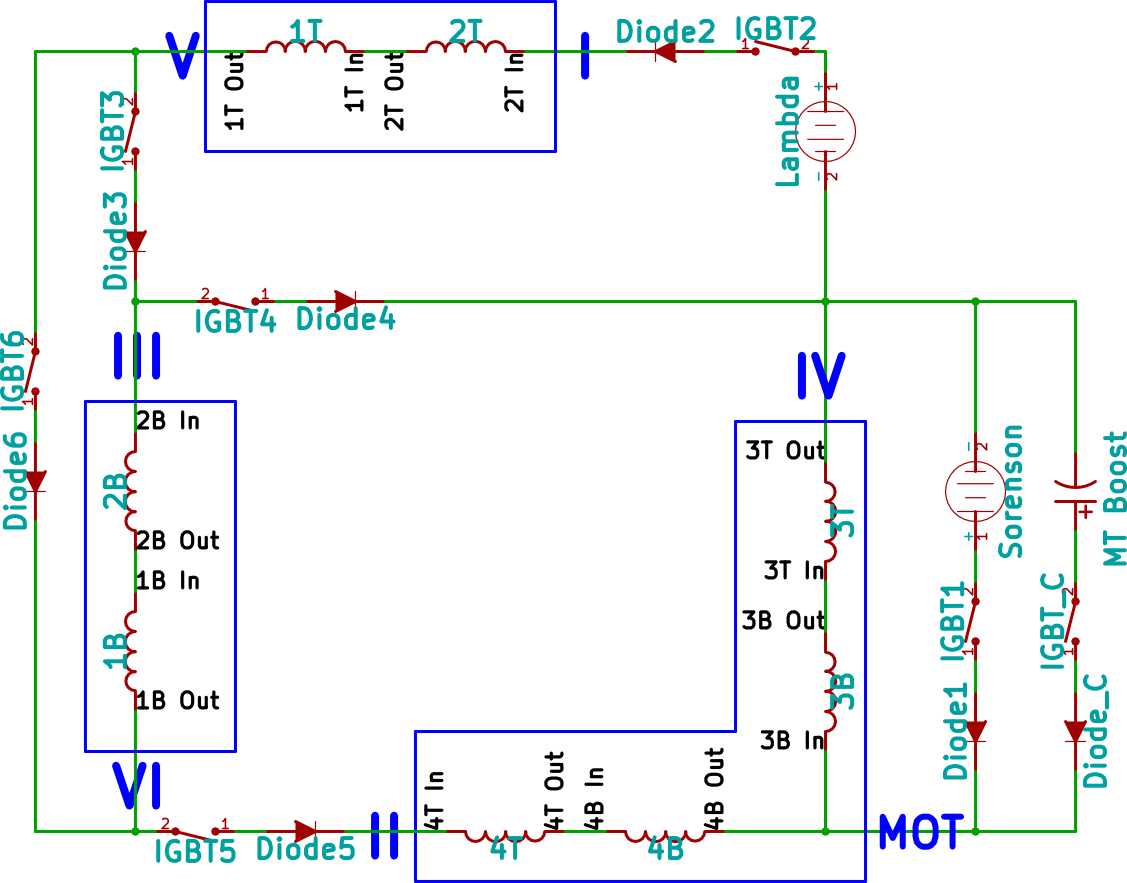
\includegraphics[width=15cm]{coil.png}
  \end{center}
  \caption{Main Coils Control Circuit. (Magnetic trap boost capacitor charging circuit not included.)}
  \label{exp:coil-control}
\end{figure}
\begin{table}
  \begin{center}
    \begin{tabular}{|c|c|c|}\hline
      \multirow{2}{*}{Closed switches(IGBTs)}& \multicolumn{2}{c|}{Usage of the power supply} \\\hhline{~--}
      &Lambda&Sorenson\\\hline
      1, 3, 5&-&\begin{tabular}{@{}c@{}}Quadrupole field with\\layer 3 for MOT and ODT\\clean up (\ref{exp:odt})\end{tabular}\\\hline
      2, 3, 5&\begin{tabular}{@{}c@{}}Quadrupole field with\\layer 1, 2, 3 and 4 for\\magnetic trap\end{tabular}&-\\\hline
      1, 2, 4, 6&\begin{tabular}{@{}c@{}}Homogeneous Feshbach resonance\\field with layer 1 and 2\end{tabular}&\begin{tabular}{@{}c@{}}Field gradient on top of\\the bias field with layer 3\\for tilt and levitation.\end{tabular}\\\hline
    \end{tabular}
  \end{center}
  \caption{List of coil configurations}
  \label{exp:coil-config}
\end{table}

\section{Magneto-Optical Trap (MOT) and Compressed-MOT}\label{exp:mot}

The MOT loading is optimized by changing the parameters of the lasers to maximize the number of atoms in the MOT after $6$ seconds of loading. The optimum settings we have found are listed in table \ref{exp:mot-param} and the performance of our MOT can be found in table \ref{exp:laser-cooling}.\\
\begin{table}
  \begin{center}
    \begin{tabular}{|c|c|c|c|c|}\hline
      MOT power&Repumper power&MOT detuning&Repumper detuning&MOT Current\\\hline
      $16$mW&$7$mW&$-38.5$mW&$-28$mW&$57$A\\\hline
    \end{tabular}
  \end{center}
  \caption{MOT parameters}
  \label{exp:mot-param}
\end{table}\\
Since our MOT is mainly optimized for loading rate, it is not necessarily optimized for density and cooling. Therefore, we added a compress-MOT (CMOT) step after the MOT in order to increase the density and decrease the temperature. In the CMOT step, we ramp the MOT frequency closer to resonance in $4.5$ms and decrease the intensity of the repumper. As a result, the cloud is compressed by radiation pressure and pumped to the $F1$ state. The temperature of the cloud is also decreased because of the decrease in scattering. Figure \ref{exp:cmot-image} shows the F pumping effect in the CMOT and the performance of the CMOT is listed in table \ref{exp:laser-cooling}.
\begin{figure}
  \begin{center}
    \subfigure[CMOT imaged with $F2$ light without $F$ pumping.]{
      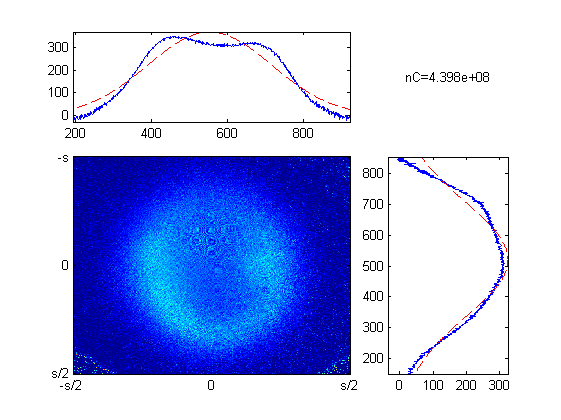
\includegraphics[width=5cm]{cmot-nopump.png}
    }
    \subfigure[CMOT imaged with $F2$ light after $F$ pump into $F2$.]{
      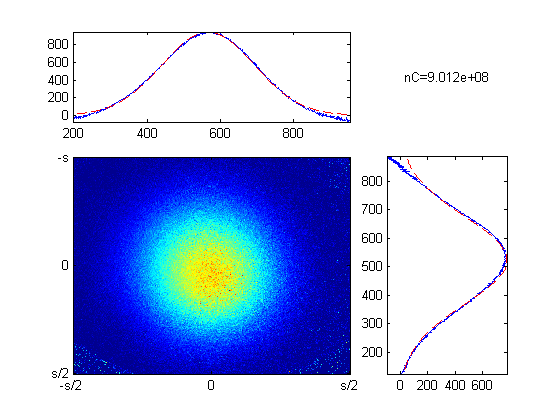
\includegraphics[width=5cm]{cmot-pump.png}
    }
  \end{center}
  \caption{Image of the CMOT. Atoms are pumped into the $F1$ states.}
  \label{exp:cmot-image}
\end{figure}

\section{Gray Molasses}\label{exp:gm}
The gray molasses step is used to cool the CMOT cloud further before transferring to the magnetic trap for evaporative cooling. As mentioned before, we use a smaller size for the gray molasses beam for higher density and better cooling performance. Since the gray molasses only works when the atoms are hit by all of the three pairs of counter-propagating beams, with a gray molasses beam size comparable to that of the cloud after CMOT (both have diameter $\approx5\text{mm}$), one of the challenging tasks for optimizing the gray molasses is to maximize the overlap between the cloud and the six beams while making sure each pairs of the beams are well aligned.\\
\\
Several strategies have been tried to align the gray molasses beams to the desired precision including overlaping with the MOT beams at far field, centering on the window of the vacuum chamber etc. However, since most of these methods relies on the geometry of the machine rather than the atom, we were not able to get the performance we want.\\
\\
In order to overcome this problem, I came up with a method to directly align the beams with the cloud after CMOT to high precision, which can achieve good alignment reliably. The idea is to image the part of the cloud that is missed by each of the beams and to use this image to center the beam on the cloud and minimizing the missing atoms number. In the experiment, this is done by first optically pump all the CMOT atoms into $F=2$ state (figure \ref{exp:gm-align-nopump}) and then shoot the cloud with a short pulse of $F=2$ light from one of the gray molasses beam path while blocking other beams (this is possible without affecting the previous steps because the MOT and gray molasses uses different beam paths). Although the atoms hit by the beam will not move so far because of the recoil, the short pulse is enough to pump them into the $F=1$ state. Therefore, imaging with $F=2$ light without a $F=1$ repumper after this will only show the atoms that are not hit by the beam. Figure \ref{exp:gm-align-before} shows one of these images for a the gray molasses beam after aligning only with the center of the chamber, in which we can clearly see shells of atoms missed by the beam. After aligning the beam with the cloud using this image, we got an image of the missing part which looks like \ref{exp:gm-align-after}. We then repeat this procedure on all the beams as well as overlaping each pair of counter-propagating beams to make sure the gray molasses is well aligned with the CMOT cloud.\\
\\
After we repeated this on all the gray molasses beams, we took time of flight images while scanning the frequencies of the light. As shown in figure \ref{exp:gm-ddet}, a clear decrease in temperature (a decrease in time of flight size) can be seen just as what we expected from the theory\ref{theory:gm} and the experimental result from other groups\cite{gm-theory}. The final performance of the gray molasses is also listed in table \ref{exp:laser-cooling}. Since the gray molasses step provide not spacial confinement, being able to maintain the same density as shown in the table confirms that the gray molasses is effecient enough to significantly cool the atoms before they fly away.
\begin{figure}
  \begin{center}
    \subfigure[CMOT atoms pumped to $F2$]{
      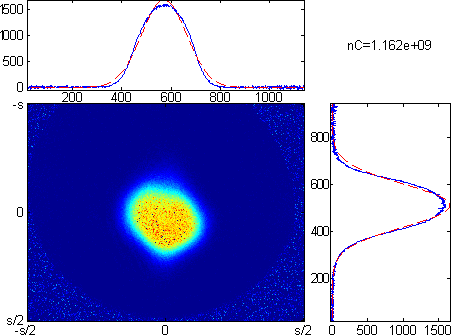
\includegraphics[width=6cm]{gm1-nopump.png}
      \label{exp:gm-align-nopump}
    }
    \subfigure[CMOT atoms pumped to $F2$ and hit with one of the gray molasses beam before alignment]{
      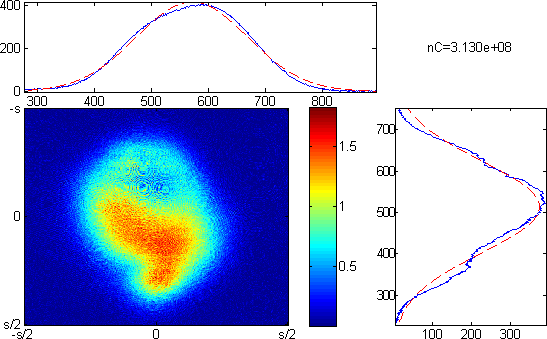
\includegraphics[width=6cm]{gm1-before.png}
      \label{exp:gm-align-before}
    }
    \subfigure[CMOT atoms pumped to $F2$ and hit with one of the gray molasses beam after alignment]{
      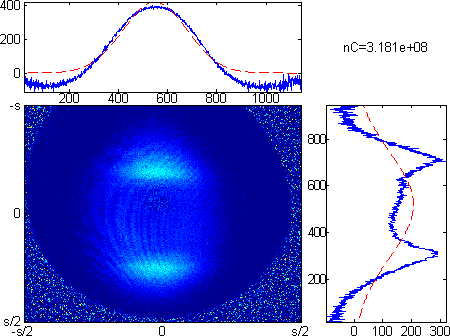
\includegraphics[width=4.5cm]{gm1-after.png}
      \label{exp:gm-align-after}
    }
  \end{center}
  \caption{Images used to align the gray molasses beams.}
  \label{exp:gm-align}
\end{figure}
\begin{figure}
  \begin{center}
    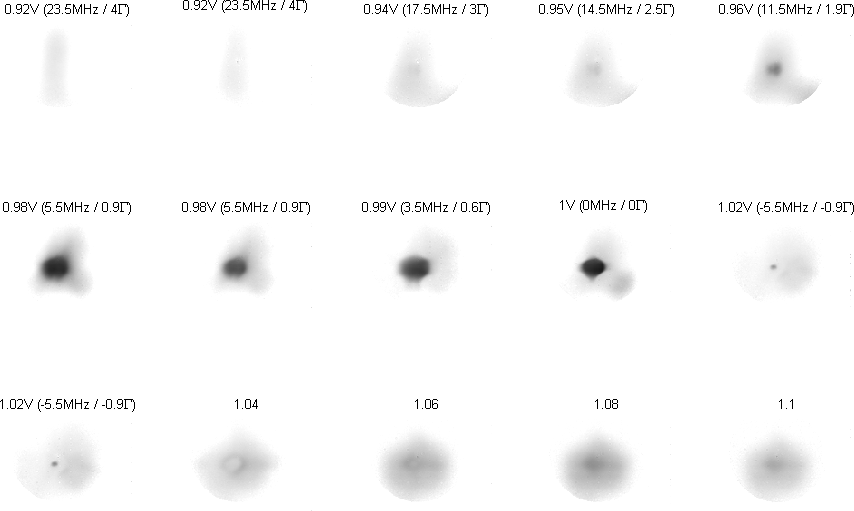
\includegraphics[width=11cm]{gm-ddet.png}
  \end{center}
  \caption{Time of flight image for gray molasses with different relative detuning (in MHz) between the pumper and repumper. (The voltages in the image is the control voltage we use to tweak the frequency.)}
  \label{exp:gm-ddet}
\end{figure}
\begin{table}
  \begin{center}
    \begin{tabular}{|c|c|c|c|c|}\hline
      Step&Atom Numbers&Temperature(K)&Density($\text{cm}^{-3}$)\\\hline
      Oven&-&$760$&-\\\hline
      Zeeman Slower&-&$0.5$&-\\\hline
      MOT&$2\cdot10^{10}$&$1.5\cdot10^{-3}$&$1\cdot10^{11}$\\\hline
      CMOT&$2\cdot10^{10}$&$1\cdot10^{-3}$&$2\cdot10^{11}$\\\hline
      Gray Molasses&$1\cdot10^{10}$&$1\cdot10^{-4}$&$2\cdot10^{11}$\\\hline
    \end{tabular}
  \end{center}
  \caption{Laser cooling performance.}
  \label{exp:laser-cooling}
\end{table}

\section{Dark State Pumping}\label{exp:pump}
At the end of Laser cooling, the atoms are distributed in different hyperfine levels not all of which are trappable. However, in order to transfer to and evaporate in the magnetic trap, all the atoms have to be in a single trappable state. The state we select in our experiment is the $F=2, m_F=2$ state both because it is trappable in any field regime and for a better elastic to inelastic collision rate ratio.\\
\\
For transfering atom into the desired state, we use the technique known as dark state pumping to minimizing the heating from photon scattering during the pumping step. Using the $D1$ transition to the $F'=2$ state, the $F=2, m_F=2$ state is dark for the $\sigma^+$ pumping light. In another word, after the atoms are pumped into the right state, they will become invisible and stop scattering any photons, in contrast with pumping with the $D2$ transition, in which case the atoms in the right state will cycle on the $F=2, m_F=2$ to $F'=3, m_F=3$ and heats up quickly.\\
\\
Another effect we want to avoid is the re-scattering of the pumping light, which happens when an atom goes into the $F=2$ state and emit a photon close to resonance with the $F=2$ transition with a random polarization that is not necessarily dark for the final state. Since the re-scattering rate is proportional to the scattering rate (i.e. pumping rate) times the scattering cross section, this effect can be minimized by increase the detuning (therefore smaller cross section) and increase the power while keeping a constant scattering rate. With the frequency range we can assess with our apparatus we blue detun the pump light by $\delta_{F1}=20\text{MHz}$ and $\delta_{F2}=34\text{MHz}$ in our experiment for the $F=1$ light and $F=2$ light respectively. Figure \ref{exp:mf-pump-time} shows the atoms after different pumping time imaged with $D1 (F=2)$ $\sigma^+$ light. The initial increase in atom number shows atoms being pumped into $F2$ and the slower decay is when they are going into the $|2, 2\rangle$ state invisible to the imaging light.
\begin{figure}
  \begin{center}
    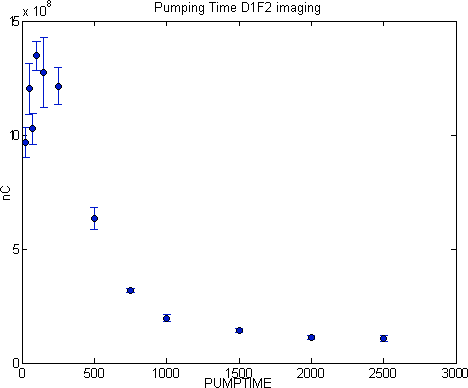
\includegraphics[width=8cm]{mf-pump.png}
  \end{center}
  \caption{Atom number imaged with $D1 (F=2)$ $\sigma^+$ light as a function of dark state pumping time.}
  \label{exp:mf-pump-time}
\end{figure}

\section{Magnetic Trap}\label{exp:mt}
In order for an atom to stay trapped in a magnetic trap, it must maintain its Zeeman level. The adiabatic condition, tells us that this means the local magnetic field of an atom should not be too small or change too fast. Although this condition can be easily satisfied for a cold enough cloud, it cannot always hold around the center of the quadrupole magnetic trap where the field goes to zero. Therefore, there is a ``hole'' at the center of a quadrupole trap where atoms can spin flip and escape and the loss caused by this ``hole'' is called Majorana loss. Since the center of the trap is also the lowest point of the trapping potential and therefore is where the atom density is maximized, we will see large Majorana lossing rate in a pure quadrupole trap. The Majorana loss can be reduced or avoided by decreasing the atom number inside the hole. In our experiment, this is done with a ``plug'' beam which is a $10$W $532$nm green laser beam focused to $20\mu m$ at the center of the trap creating a positive AC Stark shift and pushing the atoms away from the center. Figure \ref{exp:plug-power} shows the number of atom after the magnetic trap, the saturation of the atom number with $6$W of plug power shows that we have successful suppressed the Majorana loss with the plug beam.\\
\begin{figure}
  \begin{center}
    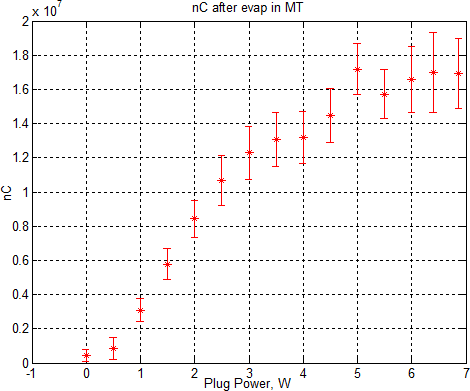
\includegraphics[width=9cm]{plug-power.png}
  \end{center}
  \caption{Saturation of the Plug Laser Power.}
  \label{exp:plug-power}
\end{figure}
\\
Due to the high three-body inelastic collision loss rate in Lithium-$7$, we need to open the trap, i.e. decrease the trapping gradient, during evaporation to keep a relatively low spacial density. However, since the center (zero) of the quadrupole field is determined by the ratio between the quadrupole field and the stray field around the center, the zero of the trap, therefore the Majorana hole, may move when we open the trap and might even move out of the plug beam. Although it is possible to shift either the zero or the plug and let them track each other during evaporation, the simplest way to solve the problem is actually to zero the stray field so that the center will never move while openning up. For achieving the high precision of field zeroing ($\leqslant100\text{mG}$), we zero the field by measuring the position of the center of the quadrupole trap. In the experiment, we decrease the trap gradient to certain value while doing a deep cut by sweeping the RF frequency close to resonance and measure the center position of the resulting small cloud left in the trap. Figure \ref{exp:field-zeroing} shows the result of this measurement with different trap gradient and bias field in both $x$ and $y$ directions. We pick the bias field with the smallest displacement at different gradient, for which the center of the trap moves by smaller than one pixel ($20\mu m$).\\
\\
Because of the small the elastic to inelastic collision rate ratio, the atom number fluctuation in the experiment and the necessity to open up the trap during evaporation, it is hard to optimize the RF evaporation purely experimentally. Instead, the evaporation in our experiment is optimized using numeric simulation. With our final sequence, after $2.5$s of RF evaporation, we are left with $6\cdot10^7$ atoms with a temperature of $4\mu$K and a density of $10^{12}\text{cm}^{-3}$.
\begin{figure}
  \begin{center}
    \subfigure[$x$ direction]{
      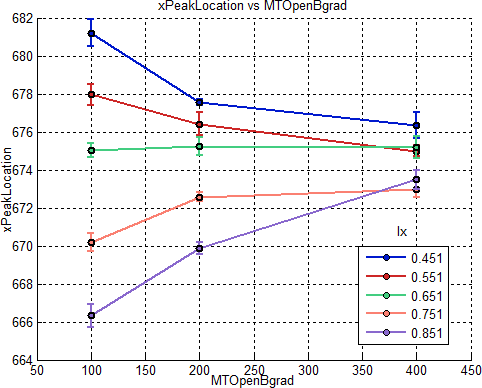
\includegraphics[width=5cm]{field-zeroing-x.png}
    }
    \subfigure[$y$ direction]{
      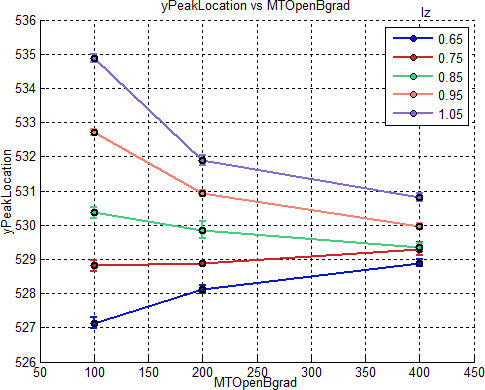
\includegraphics[width=5cm]{field-zeroing-y.png}
    }
  \end{center}
  \caption{Precise Field Zeroing in Magnetic trap}
  \label{exp:field-zeroing}
\end{figure}

\section{BEC in Optical Dipole Trap}\label{exp:odt}

After evaporation in the magnetic trap, we transfer the atoms into a optical dipole trap (ODT) created with two $15$W $1064$nm laser beams. The transfer need to be adiabatic in order to minimize heating and maximize transfer efficiency. After exploring different transfer schemes, the best method we have found is to turn on the ODT in full power before evaporating in the magnetic trap and ramp down the magnetic trap after evaporation in $200$ms. In this way, we can accumulate $2\cdot10^7$ atoms in the ODT at a temperature of $20\mu K$.\\
\\
We put the atoms from $|2, 2\rangle$ state to $|1, 1\rangle$ state using a Landau-Zener sweep with RF frequency. Figure \ref{exp:landao-zener} shows the atom number in $|2, 2\rangle$ versus starting frequency of a $1$MHz wide RF scan in a magnetic field about $1$G. We hit the resonance at $806.25$MHz and the transfer efficiency is better than $80\%$.\\
\begin{figure}
  \begin{center}
    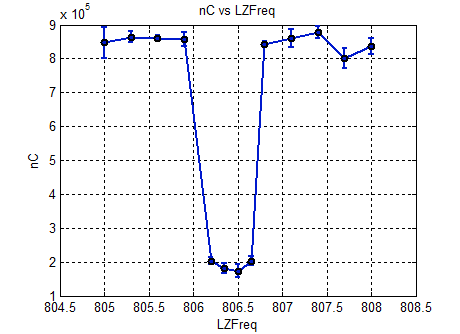
\includegraphics[width=9cm]{landao-zener.png}
  \end{center}
  \caption{Landau-Zener Sweep.}
  \label{exp:landao-zener}
\end{figure}\\
The evaporation in the ODT is aided by a Feshbach resonance. We measure the resonance using the increase in three-body loss rate. Figure \ref{exp:feshbach} shows the atom number after a certain hold time in the ODT with different Feshbach field. The resonance occurs at $285$A. By comparing the resonance point with know data for the scattering length around the resonance, we do our evaporation using a Feshbach current of $\approx275$A corresponding to a reasonably large scattering length ($\approx100a_0$).
\begin{figure}
  \begin{center}
    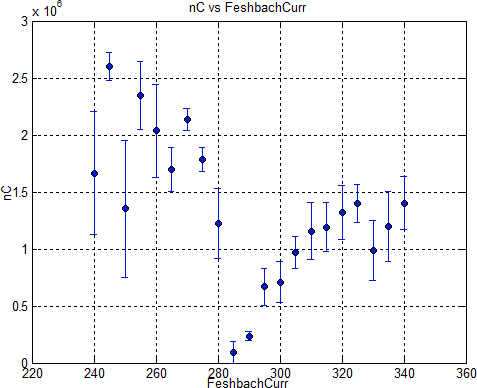
\includegraphics[width=9cm]{feshbach.png}
  \end{center}
  \caption{Feshbach Resonance in $|1, 1\rangle$ state.}
  \label{exp:feshbach}
\end{figure}

\begin{figure}
  \begin{center}
    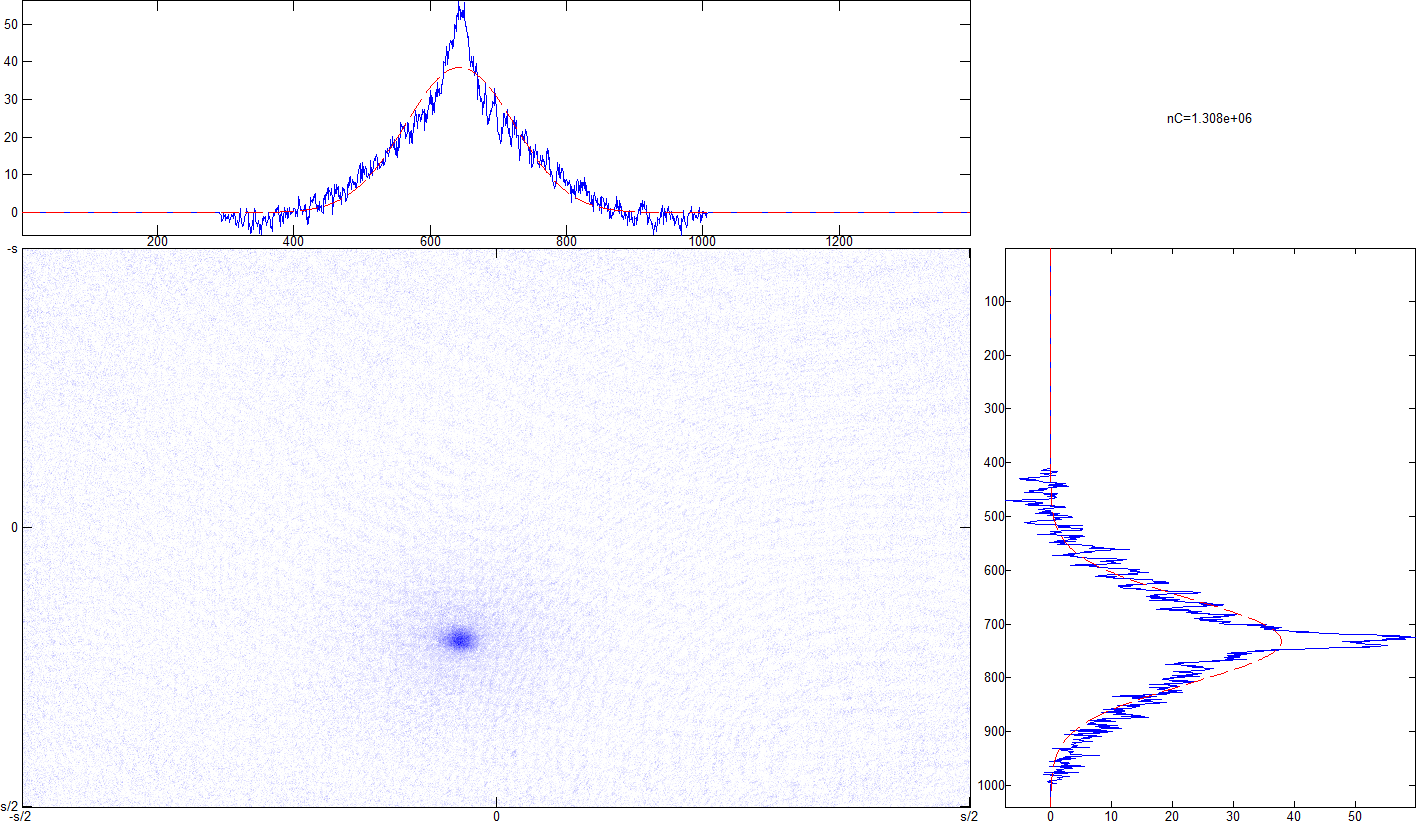
\includegraphics[width=9cm]{bec.png}
  \end{center}
  \caption{BEC with thermal wing.}
  \label{exp:bec-image}
\end{figure}

\chapter*{Conclusion}
\addcontentsline{toc}{chapter}{Conclusion}

The main goal of this work was to build an apparatus to experimentally realize a Bose-Einstein condensate which can be used as a starting point to study quantum magnetism in an optical lattice making use of the light mass and Feshbach resonance. The light mass, small elastic collision cross section and large inelastic collision loss of Lithium-$7$ makes it hard to get higher phase space density. However, as shown in the previous chapter, when the non-conventional gray molasses cooling and numerically optimized RF evaporation, we have successfully archived our goal and are able to reach quantum degeneracy within $10$ seconds including $6$ seconds of MOT loading time. We have also measured the Feshbach resonance field which is important both for evaporation in ODT and for tuning interactions in a optical lattice.\\
\\
Future work on this experiment will focus on characterizing and stabilizing our BEC and putting in the optical lattice in order to study the solid stated Hamiltonian we are interested in. Some theoretical study and intermediate steps might be necessary in order to have better understanding of our apparatus and the system we would like to study and to finallize the strategy for mapping out the quantum magnetism phase diagram.

\appendix
%% This defines the bibliography file (main.bib) and the bibliography style.
%% If you want to create a bibliography file by hand, change the contents of
%% this file to a `thebibliography' environment.  For more information
%% see section 4.3 of the LaTeX manual.
\begin{singlespace}
\bibliography{main}
\bibliographystyle{plain}
\end{singlespace}

\end{document}
